\documentclass[10pt,a4paper]{report}

\usepackage[utf8]{inputenc}
\usepackage{graphicx}
\usepackage{color}
\usepackage{cite}
\usepackage{subcaption}
\usepackage{mathtools}
\usepackage[export]{adjustbox}

\title{I love cats}
\author{Kulikov Artem}
\date{July 2022}

\begin{document}
\maketitle
\tableofcontents
\part{First part}
\chapter{Random text}
\section{I want some pizza}
\textit{Duis in sem suscipit dolor vestibulum viverra nec eget justo. Fusce ac felis a odio sodales mattis. Quisque mattis magna tellus, ut interdum nisi euismod eu. Pellentesque habitant morbi tristique senectus et netus et malesuada fames ac turpis egestas. Mauris hendrerit tortor id nibh laoreet, sed imperdiet sem rhoncus. Pellentesque lacinia commodo arcu, ac auctor lorem eleifend vel. In hac habitasse platea dictumst. Fusce sagittis ut mauris feugiat ornare. Praesent ut diam pharetra, sollicitudin elit eu, vulputate nisl. Mauris vel metus augue. In malesuada nulla quis dui porta, id luctus augue faucibus. Nullam a auctor sem.\cite{guyon2002gene}
}

\begin{figure}
    \centering
    \begin{subfigure}{0.3\textwidth}
    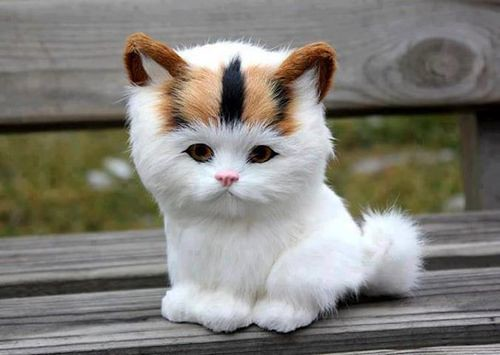
\includegraphics[width=1.1\linewidth, height=4cm]{images/2.jpg}
    \caption{cat 1}
    \label{fig:sub1}
    \end{subfigure}
    \begin{subfigure}{0.3\textwidth}
    
\includegraphics[width=1.1\linewidth, height=4cm]{images/3.jpg}
    \caption{cat 2}
    \label{fig:sub2}
    \end{subfigure}
    \begin{subfigure}{0.3\textwidth}
    
\includegraphics[width=1.1\linewidth, height=4cm]{images/4.jpg}
    \caption{cat 3}
    \label{fig:sub3}
    \end{subfigure}
    \caption{cute cats}
\end{figure}
\clearpage

\section{\footnote{I love cats.}CATS!}
Nulla faucibus tincidunt magna, id congue sapien gravida eu. In non tellus metus. Cras vel varius tortor, id feugiat sapien. Sed diam augue, vehicula a dui non, vehicula rutrum orci. Fusce vel finibus eros, a ullamcorper velit. Nullam interdum tincidunt nibh. Cras sit amet ligula sed est ultrices facilisis. Aliquam vestibulum quam vel malesuada vulputate. Duis sollicitudin mollis egestas. Fusce nec mi ac sem porttitor varius. Mauris pretium mollis suscipit. Mauris ut erat congue, lobortis magna et, condimentum dui. Pellentesque hendrerit efficitur hendrerit. Pellentesque habitant morbi tristique senectus et netus et malesuada fames ac turpis egestas \cite{guyon2002gene}
\begin{center}
\end{center}

\includegraphics[width=0.9\linewidth, right]{images/1.jpg}
\clearpage

\section{Look at this cute little thing}
Ut a semper tortor. Nulla at tristique nibh, at consectetur nunc. Nullam tempor ac diam a elementum. Interdum et malesuada fames ac ante ipsum primis in faucibus. Suspendisse potenti. Ut congue, magna gravida varius commodo, metus lacus sodales eros, sit amet maximus elit arcu at est.
WAenean eget ligula venenatis, ornare quam a, vulputate mauris. Ut non magna suscipit, convallis enim in, dictum nisi. Nullam consectetur urna at nunc suscipit, ut lobortis turpis elementum. Integer vel nisl sem. Ut at ante at arcu lobortis hendrerit. Pellentesque aliquam at diam quis rutrum. \\
\begin{figure}[h]

\includegraphics[width=\textwidth]{images/5.jpg}
\end{figure} \\
Mauris a commodo eros, ut porta enim. Cras congue efficitur ex facilisis imperdiet. Sed eget risus gravida, accumsan leo non, tempus tortor. Cras id libero neque. Sed a ullamcorper magna, id viverra tortor. Mauris at dolor quis mauris pretium suscipit sed vitae nulla. Fusce fermentum sem sit amet mollis consectetur. Sed ornare euismod dapibus. Etiam at nunc mi.\cite{noble2004support}\\

\chapter{Cats. Again. Yes}
\section{Imagine that there is a cool section name}
Mauris a commodo eros, ut porta enim. Cras congue efficitur ex facilisis imperdiet. Sed eget risus gravida, accumsan leo non, tempus tortor. Cras id libero neque. Sed a ullamcorper magna, id viverra tortor. Mauris at dolor quis mauris pretium suscipit sed vitae nulla. Fusce fermentum sem sit amet mollis consectetur. Sed ornare euismod dapibus. Etiam at nunc mi.\cite{noble2004support} \\
\begin{tabular}{c | c | c | c}
    cat & another cat & yet another cat & guess what. cat. \\ \hline
    
\includegraphics[width=0.2\textwidth, height=30mm]{images/1.jpg} & 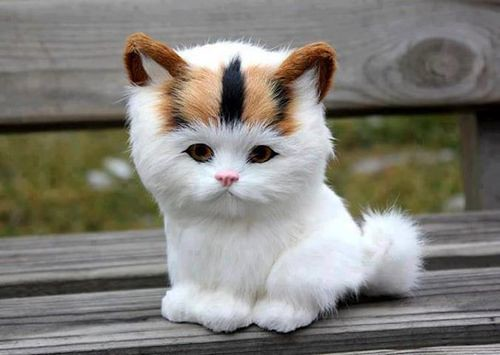
\includegraphics[width=0.2\textwidth, height=30mm]{images/2.jpg} & 
\includegraphics[width=0.2\textwidth, height=30mm]{images/3.jpg} & 
\includegraphics[width=0.2\textwidth, height=30mm]{images/4.jpg} \\
\end{tabular} \\
\begin{tabular}{c | c | c | c}
    cat & another cat & yet another cat & guess what. cat. \\ \hline
    
\includegraphics[width=0.2\textwidth, height=30mm]{images/1.jpg} & 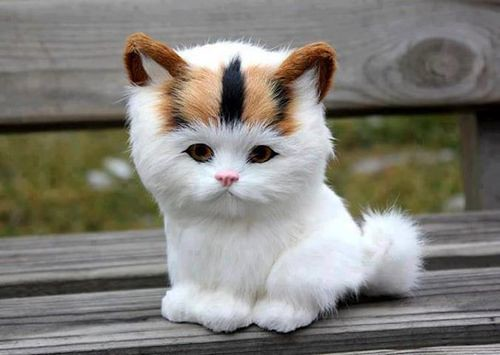
\includegraphics[width=0.2\textwidth, height=30mm]{images/2.jpg} & 
\includegraphics[width=0.2\textwidth, height=30mm]{images/3.jpg} & 
\includegraphics[width=0.2\textwidth, height=30mm]{images/4.jpg} \\
\end{tabular} \\
\begin{tabular}{c | c | c | c}
    cat & another cat & yet another cat & guess what. cat. \\ \hline
    
\includegraphics[width=0.2\textwidth, height=30mm]{images/1.jpg} & 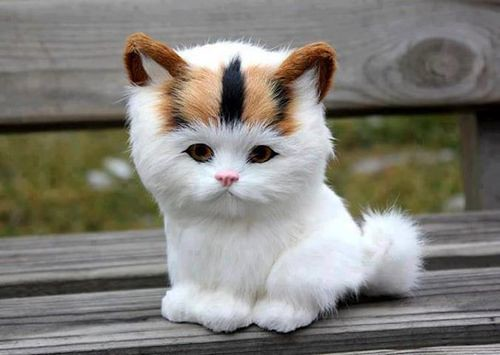
\includegraphics[width=0.2\textwidth, height=30mm]{images/2.jpg} & 
\includegraphics[width=0.2\textwidth, height=30mm]{images/3.jpg} & 
\includegraphics[width=0.2\textwidth, height=30mm]{images/4.jpg} \\
\end{tabular} \\
\clearpage
cats. cats. cats. cats. cats \\
\begin{tabular}{| r c | c |}
	\multicolumn{1}{r}{} &  \multicolumn{1}{c}{} & \multicolumn{1}{c}{} \\ \hline
	cat & 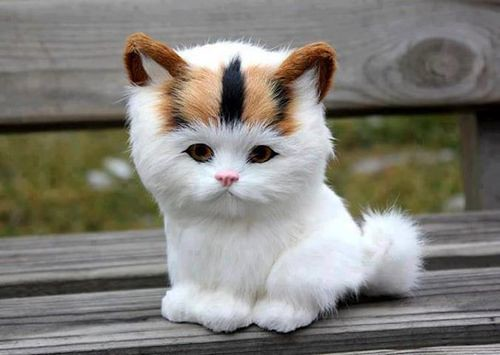
\includegraphics[width=0.2\textwidth,height=30mm]{images/2.jpg} & 
\includegraphics[width=0.2\textwidth, height=30mm]{images/1.jpg} \\ \hline
	another cat & 
\includegraphics[width=0.2\textwidth,height=30mm]{images/3.jpg} & 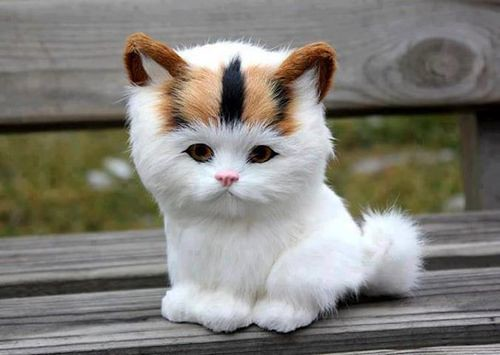
\includegraphics[width=0.2\textwidth, height=30mm]{images/2.jpg} \\ \hline
	yet another cat & 
\includegraphics[width=0.2\textwidth,height=30mm]{images/4.jpg} & 
\includegraphics[width=0.2\textwidth, height=30mm]{images/3.jpg} \\ \hline
\end{tabular} \\
\clearpage
\chapter{here go some real random things.}
\section{what is this? oh, its just cats again}

\includegraphics[width=0.2\textwidth, height=30mm]{images/1.jpg}
Unordered 
\begin{itemize}
    \item first 
    \item second
    \item third
\end{itemize} \\
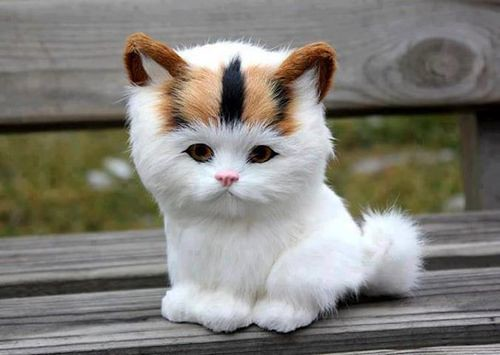
\includegraphics[width=0.2\textwidth, height=30mm]{images/2.jpg}
Ordered 
\begin{enumerate}
    \item first
    \item second
    \item third
\end{enumerate}

\includegraphics[width=0.2\textwidth, height=30mm]{images/3.jpg}
Nested 
\begin{enumerate}
    \item first
    \begin{enumerate}
        \item 1
        \item 2
        \item 3
    \end{enumerate}
    \item second
    \begin{enumerate}
        \item 1
        \item 2
        \item 3
    \end{enumerate}
    \item third
    \begin{enumerate}
        \item 1
        \item 2
        \item 3
    \end{enumerate}
    \end{enumerate}
\clearpage
\section{math thing}
\begin{align*}
    F(t)=P(Y\le t)=P(\cos(2X)\le t)=P(X\le\ 0.5 \cos^{-1}(t))=0.5 \cos^{-1}(t)? \\
\end{align*}
\begin{align*}
    H=-\left[\frac{1}{\sigma}\right]\left[g(t)f\left( k\right) +\int_{G(t)}^{1}\frac{1}{\sigma }f^{\prime }\left( \frac{t-G^{-1}(p)}{\sigma }%
+k\right) \frac{1}{g\left( G^{-1}(p)\right) }dp\right]
\end{align*}
\begin{align*}
            f'(x)           &= \lim_{h\rightarrow 0}\frac{(x+h)^{1/4}-x^{1/4}}{h}   \\
                            &=  \lim_{h\rightarrow 0}\frac{(x+h)^{1/4}-x^{1/4}}{h}\cdot \frac{((x+h)^{1/4}+x^{1/4})((x+h)^{1/2}+x^{1/2})}{((x+h)^{1/4}+x^{1/4})((x+h)^{1/2}+x^{1/2})}\\
                            &=  \lim_{h\rightarrow 0}\frac{(x+h)-x}{h((x+h)^{1/4}+x^{1/4})((x+h)^{1/2}+x^{1/2})}    \\  
                            &=  \lim_{h\rightarrow 0}\frac{1}{((x+h)^{1/4}+x^{1/4})((x+h)^{1/2}+x^{1/2})}   \\
                            &= \frac{1}{(x^{1/4}+x^{1/4})(x^{1/2}+x^{1/2})} \\
                            &=  \frac{1}{(2x^{1/4})(2x^{1/2})}  \\
                            &=  \frac{1}{4x^{3/4}}  \\
                            &=  \frac{1}{4}x^{-3/4}
\end{align*}
\begin{align*}
    a^4-b^4 &= (a^2-b^2)(a^2+b^2)   \\
        &= (a-b)(a+b)(a^2+b^2), 
\end{align*}

\bibliographystyle{plain}
\bibliography{main.bib}
  
\end{document} 



